% KansasLava-AK.tex
\begin{hcarentry}{Web Technologies}
\label{kuwebtech}
\report{Andy Gill}%11/10
\participants{Andrew Farmer, Andy Gill}
\status{ongoing}
\makeheader

At KU, we are interested in providing better support in Haskell for
interactive applications by building on top of existing web technologies,
like the fast Chrome browser, HTML5, and JavaScript. This is motivated
partly by having easy tools to teach interactive programming Haskell,
and partly by the needs of the HERMIT\cref{HERMIT} project.

Towards this, we have developed
A web request dispatch system, based on the Ruby's Sinatra, called {\tt scotty}.
(Something about being on top of the Yesod architecture, compatible, etc)

On top of {\tt scotty}, we have build a simple interface 
into the HTML5 Canvas mechanism, called {\tt blank-canvas}.
This was constructed primarily as a teaching tool, and as
a proof-of-concept of the design. Here is an example of
a teaching application which prints squares to the canvas,
based on where the user clicks the mouse.

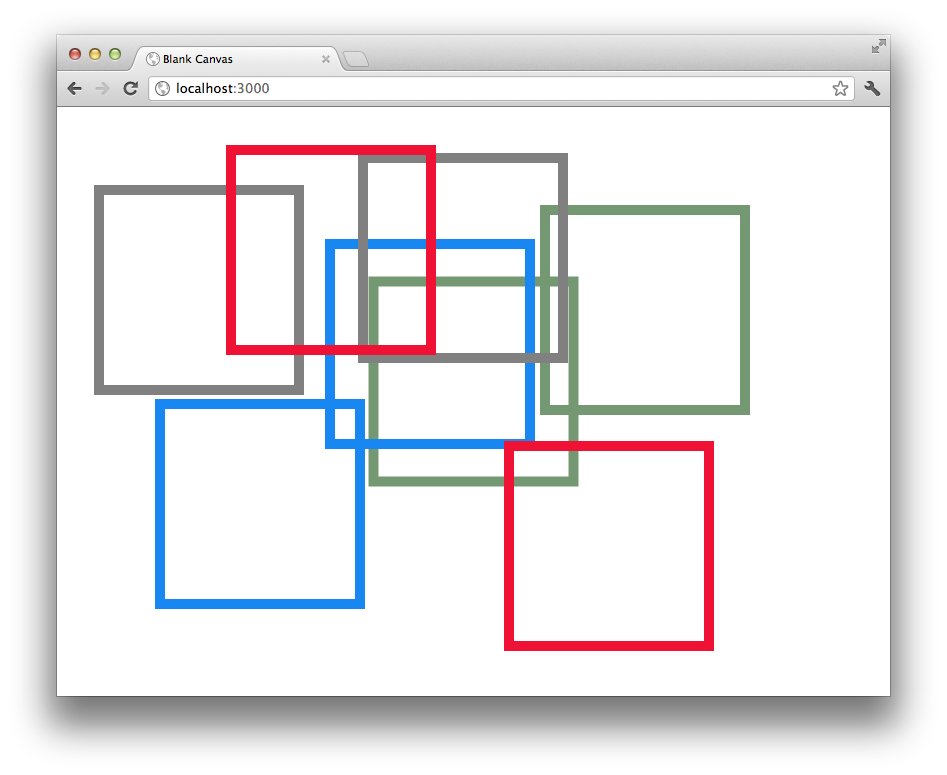
\includegraphics[width=0.47\textwidth]{html/squares.png}

Simple interactive games can be to develop using this API,
and new Haskell programmers found it straightforward to use.

The next state of a generalization of these ideas, including
a generic Javascript PUSH mechanism with asynchronous event callback support,
and the ability to support the control of arbitrary jQuery widgets within
Haskell server code.

All are available from hackage, or will be shortly. 
\end{hcarentry}
